\chapter{Evaluation}
\label{chapter:evaluation}
This chapter provides an extensive evaluation of the feasibility of using IPro as a practical approach (\textit{i.e.}, in terms of CCO, CUC, and MA) for intelligent probing in SDN. This chapter starts showing the test environment, including the SDN to monitor. After, this chapter presents the  IPro prototype developed and its impact (\textit{i.e.,} the change over the time of Probing Interval) in CCO, CUC, and MA (of the throughput) in the test environment. This chapter finishes showing the comparison of IPro with PPA and other adaptive approaches by quantitative and qualitative analysis, respectively.
\section{Setup}
\label{sec:setup}

\subsection{Test Environment}
\label{subsec:test_enviroment}

Figure~\ref{fig:campus_topo} presents the test environment used to evaluate IPro. This environment includes the campus network topology of the Federal University of Rio Grande do Sul \cite{isolani_2015:interactive}, the Ryu Controller, and the IPro prototype (\textit{cf.} Section ~\ref{subsec:prototype}). The monitored topology includes $11$ OpenFlow switches (version 1.3) that connect $230$ hosts from 7 laboratories (with 20, 30, and 40 hosts) and 4 administration offices (each one with 10 hosts) through links with a bandwidth of 10 Mbps each one. Furthermore, such topology includes a Web Server and a File Server connected in one of the administration offices. Each switch of the network is connected via a dedicated TCP channel to a remote Ryu controller used to coordinate network-wide forwarding decisions. The Mininet emulator \cite{lantz_2010:mininet} was used to deploy the monitored topology, which runs on a Ubuntu server with an Intel i7-4770 2.26 GHz and 8GB RAM. The Ryu Controller runs on a Ubuntu server with a Core i7-4770 processor and 2GB RAM.

\begin{figure}[H]
    \centering
    \includegraphics[width=0.75\columnwidth]{figures/Fig4-topology}
    \caption{Test Environment}
    \label{fig:campus_topo}
\end{figure}

To reliably test IPro, a realistic evaluation framework reflecting current and forecasted traffic patterns (\textit{e.g.,} web, P2P, and video) was used. In this master dissertation, to two measurement studies that investigate the composition of realistic traffic patterns \cite{labovitz_2011:interdomain, maier_2009:dominant} was resorted. The results indicate the dominance of Web traffic, amounting to 52\% overall measured traffic, followed by video traffic with 25-40\% of all traffic, while P2P traffic constituting only 18.3\% of total traffic. Thus, in all experiments, only Video and Web traffic was generated, in a proportion of 75\% to 25\%, respectively.\\

The Video traffic was generated by using the VLC media player \cite{Muller:2011:VMP:2072298.2072429} that can be used as a server and as a client to stream and receive video streams. The Web traffic was generated by using the Apache Server \cite{Mockus:2000:CSO:337180.337209} and http-clients based on Linux wget. These servers and clients were included in the campus topology. In this evaluation was assumed that all 230 hosts are active during the whole experiment time and place a request on average every 30 seconds. Furthermore, all experiment results have a confidence level equal to or higher than 95\%.
\subsection{Prototype}
\label{subsec:prototype}

Figure~\ref{fig:prototype_ipro} depicts the IPro prototype including: \textit{RL-agent}, \textit{Data Processing}, \textit{Flow Statistics Collection}, \textit{Data Repository}, \textit{Probing Manager}, \textit{Query Manager}, and \textit{Statistics Module}. \textit{RL-agent} and \textit{Data Processing} were developed and deployed using version 1.15 of Numpy that is the fundamental Python package for scientific computing. \textit{Probing Manager}, \textit{Query Manager}, and \textit{Statistics Module} were developed using the REST-based API provided by Ryu. This API helps to retrieve the switch statistics. \textit{Flow Statistics Collection} was developed using the Ryu API based on Python. \textit{Data Repository} was developed in MySQL. The IPRo prototype (including all test scripts) is available in \cite{castillo:ipro}.

\begin{figure}[H]
    \centering
    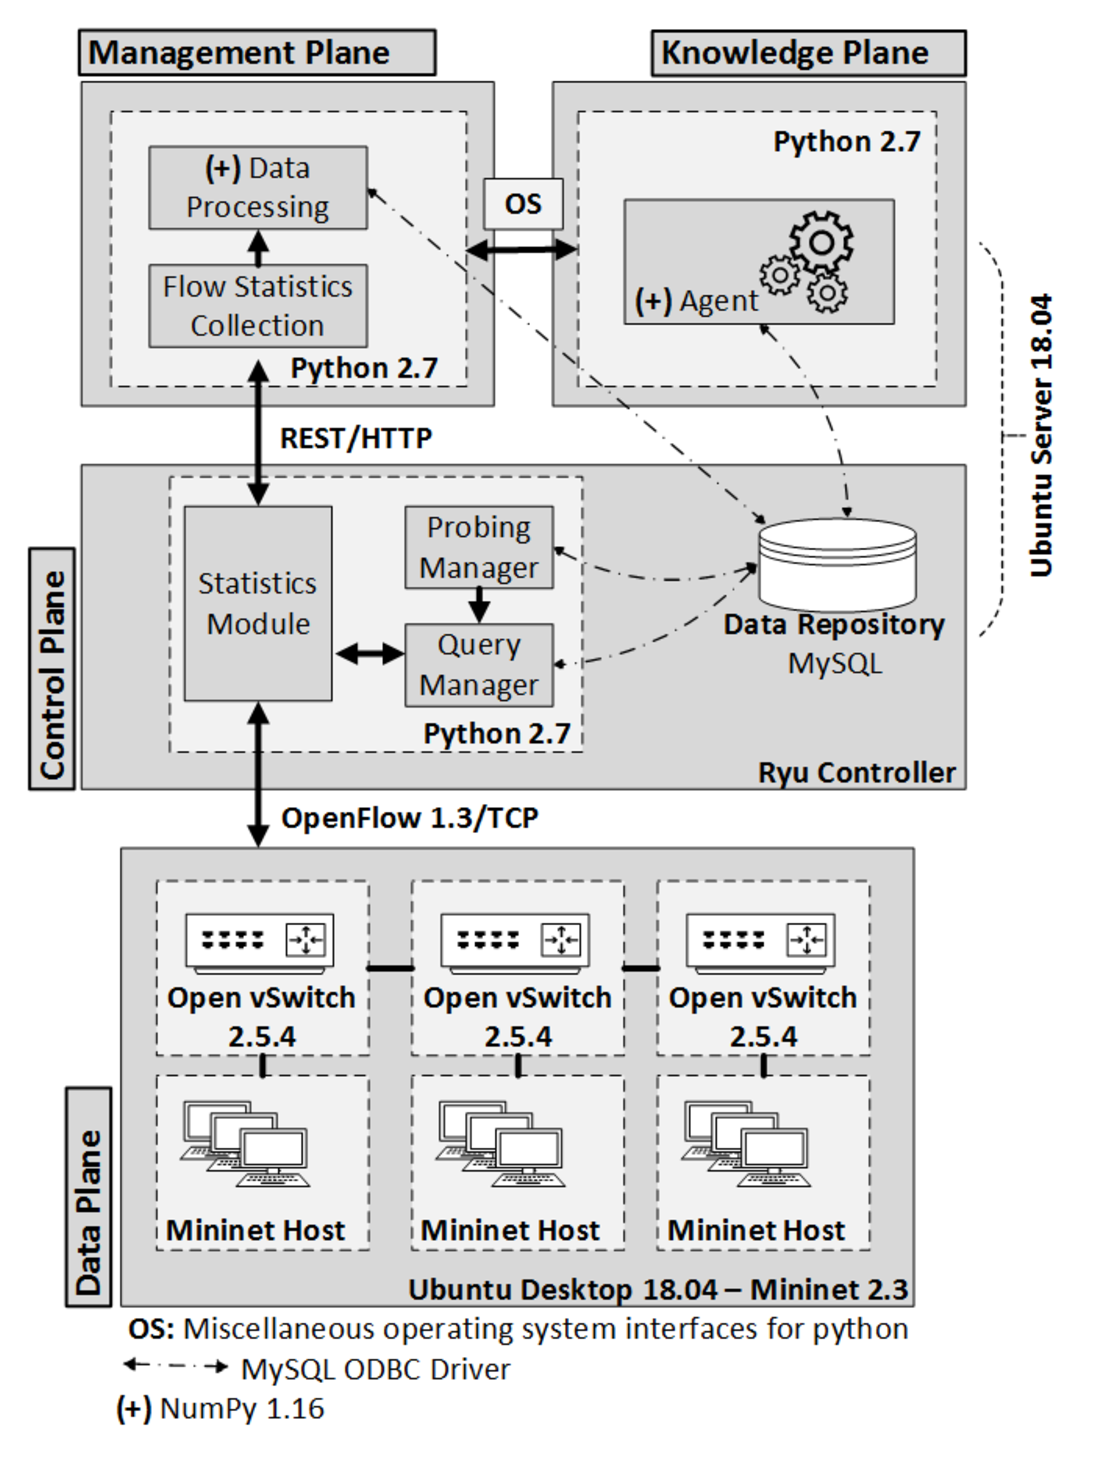
\includegraphics[scale=0.5]{figures/Fig5-IPro-prototype}
    \caption{IPro - Prototype}
    \label{fig:prototype_ipro}
\end{figure}

It is important to highlight that the \textit{Statistics Module} interacts with DP by the OpenFlow Protocol \cite{onf_2012:openflow}. This protocol was used because it has progressively turned on the SBI \textit{de-facto} standard in SDN \cite{nunes_2014:survey_past_present_future}. OpenFlow describes an open protocol that allows software applications to program (\textit{i.e.}, add, update, and delete flow entries) the flow table of the OpenFlow-compliant switches. In particular, the \textit{Statistics Module} uses the OpenFlow version 1.3. Specifically, this module uses two Read-State (Request-Reply) messages to collect information from the switch, such as current configuration, statistics, and capabilities. The controller sends a Read-State Request message to the switches to request the traffic statistics of flows. The switches communicate to the controller the requested traffic statistics via Read-State Reply messages. To get OpenFlow details,  the reader to Openflow specification is refered \cite{onf_2012:openflow}.

\subsection{Space of States}
\label{subsec:space_states}

To determine the finite space of states (\textit{cf}. Equation~\ref{equ:states_model}) that the IPro RL-agent needs to operate, first, the CCO (\textit{cf}. Equation~\ref{equ:load}), CUC (\textit{cf}. Equation~\ref{equ:load_cpu}), and MA (\textit{cf}. Equation~\ref{equ:ma}) were estimated and experimentally measured when the probing interval varies. The probing intervals between 1 and 15 seconds were manually tested (in steps of 1 second). For each interval, the test duration was 600 seconds. Second, the CCO and CUC were discretized by using the obtained results.

\subsubsection{Control Channel Overhead}
Aiming at determining the space of states that the IPro RL-agent needs to operate, Figure~\ref{fig:control_channel_load_behavior} presents the impact of the probing intervals on CCO. If the network is monitored with a probing interval upper or equal than 5 seconds, the overhead is lower than 12\%. When this interval is smaller than 5 seconds the overhead increases (top than 20\%) due to the big size and quantity of Read-State (Request-Reply) messages (\textit{cf}. Equation~\ref{equ:load}). These results corroborate that the probing interval affects CCO significantly.

\begin{figure}[h!]
    \centering
    \includegraphics[width=1.0\textwidth]{figures/Fig7-control-channel-behavior}
    \caption{CCO Variation}
    \label{fig:control_channel_load_behavior}
\end{figure}

\subsubsection{CPU Usage of the Controller}
Aiming at determining the space of states that the IPro RL-agent needs to operate, Figure~\ref{fig:cpu_behavior} presents the impact of the probing intervals on CUC. If the network is monitored with a probing interval upper or equal than 5 seconds, CUC increases on average 8.5\% approximately. Nevertheless, when this interval is smaller than 5 seconds, CUC increases (top than 20.5\%) because the controller collects statistics information more frequently. As a consequence, the controller CPU must process a higher amount of instructions per second for (de)fragmenting and reading the Read-State messages. Overall, these results corroborate that the probing interval can affect CUC significantly.

\begin{figure}[h!]
    \centering
    \includegraphics[width=1.0\columnwidth]{figures/Fig6-cpu-usage}
    \caption{CUC Variation}
    \label{fig:cpu_behavior}
\end{figure}

\subsubsection{Monitoring Accuracy}

\begin{figure}[h!]
    \centering
    \includegraphics[width=1.0\columnwidth]{figures/Fig9-throughput}
    \caption{MA of throughput }
    \label{fig:throughput}
\end{figure}

To evaluate MA, the throughput metric was measured in each probing interval and determine its respective accuracy using Equation~\ref{equ:ma}. Figure~\ref{fig:throughput} depicts the evaluation results, disclosing that MA in the throughput measured is higher than 80\% when the probing interval varies between 4 and 6 seconds. In particular, the interval of 5 seconds reports the highest MA (88.83\%). In turn, the intervals of 6 seconds and 4 seconds achieve an MA equal to 86.06\% and 83.83\%, respectively. Nonetheless, MA reduces considerably for the other probing intervals. For instance, the interval of 7 seconds accomplishes an MA lower than 69.93\% due to the reduction in the quantity of collected information. In turn, the probing intervals 1, 2, and 3 seconds lead to high CCO that interferes with SDN management messages. Furthermore, these intervals also lead to high CUC that compromises the correct operation of the controller and, so, of the underlying data plane. These two facts deteriorate the correct operation of the network generating high TCP errors and low processing of SDN management messages (\textit{cf}. Figure~\ref{fig:tcp-erros}). Therefore, the MA of data collected is also affected. In summary, the above results corroborate that the probing interval affects MA significantly.

\begin{figure}[h!]
    \centering
    \includegraphics[width=1.0\textwidth]{figures/Figure9b-tcp-errors}
    \caption{TCP errors generated by Monitoring Interference}
    \label{fig:tcp-erros}
\end{figure}

\subsubsection{Spaces Discretization}
Since IPro is RL-based, it models its environment as a finite MDP. In order to get a finite space of states, the CCO and CUC were discretized by using the results above presented (\textit{cf.} Figures~\ref{fig:control_channel_load_behavior} and ~\ref{fig:cpu_behavior}) as follows:

\begin{enumerate}
    \item The values of CCO and CUC are represented in the interval $\left [ 0,1 \right ]$, where 0 represents 0\% and 1 represents 100\%.
    \item The policy 1 (related to the threshold $\omega$) is set to 80\% aiming at preventing response times of controller upper than 1 millisecond \cite{repas_2015:performance_cpu}. Thus, \\
    CCO: $ l =\left \{ \left [ 0,0.4 \right ), \left [ 0.4,0.5 \right ), \left [ 0.5,0.6 \right ), \left [ 0.6,0.7 \right ) ,\left [ 0.7,0.8 \right )\right \}$.
    \item The policy 2 (related to the threshold $\chi$) is set to 80\% targeting to avoid interference with essential SDN functions (\textit{e.g.}, packet forwarding and route updating) and the reduction of network performance \cite{xu_2017:wildcard_requests}. Thus, \\
    CUC: $cpu=\left \{ \left [ 0,0.4 \right ),\left [ 0.4,0.5 \right ),\left [ 0.5,0.6 \right ),\left [ 0.6,0.7 \right ),\left [ 0.7,0.8 \right ) \right \}$.
    \item The Probing Interval: $i = \left \{\left [ 4,10 \right ] \right \}$. 
\end{enumerate}

It is important to highlight that CCO and CUC can be divided into smaller sub-intervals to facilitate the RL-agent decision making process. However, smaller intervals increase the size of the space of states and, so, slow down the learning process convergence rate. Thus, the discretized space of states is:

{\setlength{\mathindent}{3cm}
\begin{equation}
    \begin{split}
      S\equiv f\left ( i, l, cpu \right ): & i\in \left [ 4,10 \right ], l=\left \{ 0,0.4,0.5,0.6,0.7,0.8 \right \},\\ 
      & cpu=\left \{ 0,0.4,0.5,0.6,0.7,0.8 \right \} 
    \end{split}
    \label{equ:states}
\end{equation}
}
\section{Intelligent Probing Behavior}
\label{sec:ipro_behavior}

To evaluate the IPro prototype (\textit{cf}. Algorithm 3), its impact (\textit{i.e.,} the change over the time of Probing Interval) in CCO, CUC, and MA (of the throughput) was tested in the test environment described in Section~\ref{sec:setup}. Figure~\ref{fig:load_behavior} depicts the evaluation results, disclosing diverse facts.

%\begin{figure}[htb]
\begin{figure}[h!]
\centering
        \begin{minipage}[t]{1.0\textwidth}
            \centering
            \includegraphics[width=\textwidth]{figures/Figure12a-IPro-behavior-MA-CCO-CUC}
            %\subcaption{Image 1.}\label{fig:1}
        \end{minipage}
        \hfill
        \begin{minipage}[t]{1.0\textwidth}
            \centering
            \includegraphics[width=\textwidth]{figures/Figure12b-IPro-behavior-MA-CCO-CUC}
            %\subcaption{Image 2.}\label{fig:2}
        \end{minipage}
        \vspace{-0.5cm}
        \caption{Behavior of the CCO, CUC, MA, and Probing Interval}
        \label{fig:load_behavior}
\end{figure}

\begin{itemize}
    \item During the first 238 seconds (convergence time), CCO, CUC, and MA present a highly fluctuating behaviour Figure~\ref{fig:load_behavior}(a,b,c). This behaviour is because the RL-agent does not have a previous knowledge (\textit{i.e.}, the Q-function starts empty and is filled during this time). Therefore, it is necessary that such an agent starts the exploration process to determine the effect of each action on the network status (\textit{i.e.}, learning process). Figure~\ref{fig:load_behavior}(d) illustrates how the Probing Interval changes during the learning process. As the learning process advances, the RL-agent visits each state of the space of states (\textit{cf.} Equation~\ref{equ:states}) multiple times aiming at finding the most-rewarding probing strategy (\textit{i.e.}, the convergence of the learning process).
    \item After the convergence time, IPro has a CCO near to 1.23\%, a CUC around 7.4\%, and a MA about 96\%. This result demonstrates that, in terms of CCO, CUC, and MA, IPro has good behavior. When the learning process tends to converge, the fluctuations of CCO, CUC, and MA decrease to a smaller radius. This convergence is because a normal distribution function (\textit{cf}. Equation~\ref{equ:reward}) was chosen whereby IPro gradually moves to adjacent states to the target state (\textit{i.e.}, calibrates the action-value function). In particular, IPro provides the best behaviour regarding CCO, CUC, and MA when it probes the network with intervals between 4 and 6 seconds.
    \item It is important to highlight that IPro does not stop its learning because, in real networks, the environment will always be changing and evolving.
\end{itemize}

To determine the performance of IPro itself, the consumption of CPU and memory of its RL-agent was evaluated. Figure~\ref{fig:rl-agent_behavior} depicts the evaluation results, disclosing that this RL-agent does not consume intensively the KP resources, approximately 1\% -2\% of CPU and 30MBytes. These results demonstrate that, in terms of CPU and memory, IPro RL-agent is efficient.

\begin{figure}[h!]
    \centering
    \includegraphics[width=1.0\textwidth]{figures/Figure13-cpu-usage-rl-agent}
    \caption{Behavior of the CPU usage and memory of RL-agent}
    \label{fig:rl-agent_behavior}
\end{figure}
\section{Comparison}
\label{sec:ipro_performance}
IPro was compared to PPA (\textit{i.e.,} a pull-based approach targeted to monitor the network switches with a pre-defined probing interval) regarding CCO, CUC, and MA after and before the convergence time. The probing intervals tested were ranging between 1 and 15 seconds (in steps of 1 second). For each interval, the test was performed 32 times during 600 seconds (the initial 238 seconds correspond to convergence time), aiming at obtaining the average of CCO, CUC, and MA. Next, only the 4, 5, and 6 seconds probing intervals was analyzed because, in them, the MA of measurements of both throughput and delay metrics is higher than 80\%. Finally, the comparison of IPro with other adaptive approaches was extended by a qualitative analysis.

\subsection{After Converging}
\label{converge}

\fontsize{7}{8}\selectfont
{\renewcommand{\arraystretch}{1.4}
\begin{table*}[!htp]
\scriptsize
\begin{center}
\footnotesize
\begin{tabularx}{\linewidth}{P{30mm}P{30mm}P{28mm}P{28mm}P{28mm}}
\hline
\textbf{\rotatebox[origin=c]{0}{Probing }}& \textbf{\rotatebox[origin=c]{0}{MA of}} &\textbf{\rotatebox[origin=c]{0}{MA of}}&\textbf{\rotatebox[origin=c]{0}{CUC [\%]}}&\textbf{\rotatebox[origin=c]{0}{CCO [\%]}}\\[-2ex]
\textbf{\rotatebox[origin=c]{0}{Interval [s] }}& \textbf{\rotatebox[origin=c]{0}{Throughput [\%]}} &\textbf{\rotatebox[origin=c]{0}{Delay [\%]}}&\textbf{\rotatebox[origin=c]{0}{}}&\textbf{\rotatebox[origin=c]{0}{}}\\\hline

\rowcolor{gray!20} IPro  &  96.17 & 94.78&  7.40 & 1.23  \\\hline
PPA with 4     &  83.59 &  82.50&   20.60 & 17.40  \\\hline
PPA with 5     &  91.38 &  89.50&   11.70 & 11.45  \\\hline
PPA with 6     &  86.35 &  81.03&   10.10 & 11.33  \\\hline
\end{tabularx}
\caption{Comparison after converging}
\label{tab:results_comparison_after}
\end{center}
\end{table*}
}
\normalsize

After converging (\textit{i.e.,} the RL-agent has learned), the experimental results (\textit{cf.} Table~\ref{tab:results_comparison_after}) reveal diverse facts related to the use of RL for tuning the probing interval:

\begin{itemize}
    \item IPro has a CCO significantly smaller than PPA. The reduction in the intervals of 4, 5, and 6 seconds is around 16.17\%, 10.22\%, and 10.1\%, respectively.
    \item IPro uses better the CPU of the controller than PPA about 13.2\%, 4.3\%, and 2.7\%, respectively.
    \item IPro achieves a higher MA when used to measure the throughput metric than PPA about 12.58\%, 4.79\%, and 9.82\%, respectively.
    \item IPro achieves a higher MA when used to measure the delay metric than PPA about 12.28\%, 5.28\%, and 13.75\%, respectively.
\end{itemize}{}

These facts are because, at each time step, IPro uses the network state for improving its control policies and, then, takes the best action based on the improved policies. These policies lead to better monitoring regarding CCO and CUC. To sum up, the RL-agent of IPro provides a good behavior in CCO and CUC without compromising MA.

\subsection{Before Converging}

\fontsize{7}{8}\selectfont
{\renewcommand{\arraystretch}{1.4}
\begin{table*}[!htp]
\scriptsize
\begin{center}
\footnotesize
%\rowcolors{1}{lightgray}{white}
\begin{tabularx}{\linewidth}{P{30mm}P{30mm}P{28mm}P{28mm}P{28mm}}
\hline
\textbf{\rotatebox[origin=c]{0}{Probing }}& \textbf{\rotatebox[origin=c]{0}{MA of}} &\textbf{\rotatebox[origin=c]{0}{MA of}}&\textbf{\rotatebox[origin=c]{0}{CUC [\%]}}&\textbf{\rotatebox[origin=c]{0}{CCO [\%]}}\\[-2ex]
\textbf{\rotatebox[origin=c]{0}{Interval [s] }}& \textbf{\rotatebox[origin=c]{0}{Throughput [\%]}} &\textbf{\rotatebox[origin=c]{0}{Delay [\%]}}&\textbf{\rotatebox[origin=c]{0}{}}&\textbf{\rotatebox[origin=c]{0}{}}\\\hline

\rowcolor{gray!20} IPro  &  85.58 & 84.60 &  7.56 & 1.23  \\\hline
PPA with 4     &  87.05 &  85.30&   22.32 & 17.40  \\\hline
PPA with 5     &  90.63 &  91.50&   10.12 & 11.45  \\\hline
PPA with 6     &  89.44 &  86.02&   11.08 & 11.33  \\\hline
\end{tabularx}
\caption{Comparison before converging}
\label{tab:results_comparison_before}
\end{center}
\end{table*}
}
\normalsize
Before converging (\textit{i.e.,} the RL-agent is learning), the experimental results (\textit{cf.} Table~\ref{tab:results_comparison_before}) reveal diverse facts related to the use of RL for tuning the probing interval. 

\begin{itemize}
    \item IPro achieves a smaller MA in the throughput measurement than PPA, about 1.44\%, 5.05\%, and 3.86\% in the intervals of 4, 5, and 6 seconds, respectively.
    \item IPro achieves a smaller MA in the delay measurement than PPA, about 0.7\%, 6.9\%, and 1.42\%, respectively.
\end{itemize}{}

These facts are because, in this period, IPro explores the effect of each action on the network status (\textit{i.e.,} learning process). To sum up, IPro requires a time to capture the environment model before converging to the optimal policy. Conversely, as presented in Section~\ref{converge}, when the RL-agent converges to the optimal policy; it gets the most-rewarding probing interval that minimizes the performance degradation (regarding CCO and CUC) caused by monitoring tasks and improving MA (regarding throughput and delay).\\

\subsection{Qualitative Analysis}

\fontsize{9}{8}\selectfont
\begin{table*}[!htp]
\begin{center}
\scriptsize
\begin{longtable}{P{0.5cm}|P{0.2cm}|P{0.2cm}|P{0.2cm}|P{0.2cm}|P{0.2cm}|P{11.4cm}}
%\begin{longtable}{P{0.8cm}|P{0.2cm}|P{0.2cm}|P{0.2cm}|P{0.2cm}|P{7.8cm}X}
\caption{Comparison between IPro and other adaptive methods -- H $\rightarrow$ High and L $\rightarrow$ Low} \\
\hline
\multicolumn{1}{c|}{\textbf{Work}}& \multicolumn{1}{c|}{\textbf{\rotatebox[origin=c]{90}{Adaptive}}} & \multicolumn{1}{c|}{\textbf{\rotatebox[origin=c]{90}{Accuracy}}} & \multicolumn{1}{c|}{\textbf{\rotatebox[origin=c]{90}{Overhead}}} & \multicolumn{1}{c|}{\textbf{\rotatebox[origin=c]{90}{CPU}}} & \multicolumn{1}{c|}{\textbf{\rotatebox[origin=c]{90}{ML}}} & \multicolumn{1}{c}{\textbf{\rotatebox[origin=c]{0}{Description}}} \\ 
\hline 
\endfirsthead

\multicolumn{7}{c}%
{{\bfseries \tablename\ \thetable{} -- Continued from previous page}} \\
\hline 
\multicolumn{1}{c|}{\textbf{Work}}& \multicolumn{1}{c|}{\textbf{\rotatebox[origin=c]{90}{Adaptive}}} & \multicolumn{1}{c|}{\textbf{\rotatebox[origin=c]{90}{Accuracy}}} & \multicolumn{1}{c|}{\textbf{\rotatebox[origin=c]{90}{Overhead}}} & \multicolumn{1}{c|}{\textbf{\rotatebox[origin=c]{90}{CPU}}} & \multicolumn{1}{c|}{\textbf{\rotatebox[origin=c]{90}{ML}}} & \multicolumn{1}{c}{\textbf{\rotatebox[origin=c]{0}{Description}}} \\
\hline 
\endhead

\hline \multicolumn{6}{r}{{Continued on next page}} \\ \hline
\endfoot

\hline \hline
\endlastfoot

\RaggedRight IPro & \checkmark & H & L & L & \checkmark & \justifying\noindent{An RL-based algorithm is used to get an optimal probing interval to achieve a trade-off between MA, CCO, and CUC} & \hline
%###################################### First Stream ###################################################################
\RaggedRight \cite{chowdhury_2014:payless}& \checkmark & H & H & H &  & \justifying\noindent{Adaptive sampling algorithms are used to tune the load level generated by monitoring process} & \hline

\RaggedRight \cite{raumer_2014:monsamp}& \checkmark & H & H & H &  & \justifying\noindent{Thresholds are used to adjust the load level generated by monitoring process} & \hline

\RaggedRight \cite{van_2014:OpenNetMon}& \checkmark & H & H & H &  & \justifying\noindent{An adaptive fetching mechanism monitors per-flow metrics, such as throughput, delay, and packet loss} & \hline

\RaggedRight \cite{tahaei_2017:multi-objective}& \checkmark & H & L & L &  & \justifying\noindent{An adaptive flows statistical collection method is used to adjust the polling intervals} & \hline

%###################################### Second Stream ###################################################################
\RaggedRight \cite{jose_2011:online_measurement}& \checkmark & H & L & L &  & \justifying\noindent{A small set of matching rules and secondary controllers are used to identify and monitor aggregate flows} & \hline

%###################################### Third Stream ###################################################################

\RaggedRight \cite{Tangari_2018:adaptive_decentralized_monitoring}& \checkmark & H & L & L &  & \justifying\noindent{A self-tuning monitoring mechanism is used to automatically adapt its settings based on the traffic dynamism} & \hline

\RaggedRight \cite{phan2017:adaptive_sdn_mon}& \checkmark & H & L & H &  & \justifying\noindent{Extra modules are included in the switches to distribute the monitoring tasks in a balanced way} & \hline

\RaggedRight \cite{tahaei_2018:cost_effective}& \checkmark & H & L & L &  & \justifying\noindent{A two layers hierarchy of controllers is described. The lowest layer polls the flow statistic and forwards statistics to the top layer. The highest layer coordinates the controllers located at the lowest level}
\label{tab:comparison-adptive-probing} & \hline
\end{longtable}
\end{center}
\end{table*}
\normalsize

Table~\ref{tab:comparison-adptive-probing} presents a qualitative comparison between IPro and other adaptive methods, disclosing diverse facts. 

\begin{itemize}
    \item Methods such as \cite{chowdhury_2014:payless, raumer_2014:monsamp, van_2014:OpenNetMon} obtain accurate measurements using adaptive techniques and threshold-based methods at expenses of increasing CCO and CPU usage (\textit{i.e.}, imbalance between MA and CCO/CPU). IPro offers an RL-based algorithm that obtains accurate measurements with CCO and CPU usage negligible (\textit{i.e.,} achieves a trade-off between MA, CCO, and CUC).
    
    \item Methods such as \cite{jose_2011:online_measurement, Tangari_2018:adaptive_decentralized_monitoring, phan2017:adaptive_sdn_mon, tahaei_2018:cost_effective} obtain accurate measurements with low overhead using distributed controllers. These methods differ significantly from IPro. Whereas goal IPro is to optimize the probing interval, these methods focus on merges the collected statistics by every controller in an only statistic metric. 
    
    \item None of these adaptive approaches consider ML-bases mechanisms that optimize such a trade-off by learning from the network behavior, causing potential bottlenecks in the control channel, packet/flow loss, and performance drops.
\end{itemize}{}

Finally, in this qualitative analysis, it is essential to highlight two facts. The first one, the convergence time is an intrinsic parameter of RL-based approaches. The RL-agent exploits known actions to obtain a reward and explores new ones to make better decisions. This agent tries a variety of actions to progressively favor those that appear to be the best. The exploration and exploitation principles introduce a challenge related to the balance between them, which is known as the exploration-exploitation dilemma. This master dissertation does not address this challenge. Indeed, in the IPro prototype,  the e-greedy exploration method was used and did not test another one. Second, the learning time of any RL-agent depends mainly on the size of the space of states; due to it, this master dissertation used a finite one.

\section{Final Remarks}
\label{sec:final_remarks_kap5}

This chapter presented the test environment used to evaluate IPro, its prototype, and the evaluation. To reliably evaluate IPro, a realistic evaluation framework was used reflecting current and forecasted traffic patterns ( e.g., web, P2P, and video). In all experiments, only video and Web traffic were generated, in a proportion of 75\% to 25\%, respectively (given that the size of the video requests generates more traffic than web requests. Furthermore, all experiment results have a confidence level equal to or higher than 95\%. Such evaluation was carried out in terms of the following metrics: CCO, CUC, and MA. \\

The evaluation results revealed several facts:
\begin{itemize}
    \item IPro has a CCO significantly smaller than PPA. The reduction in the intervals of 4, 5, and 6 seconds is around 16.17\%, 10.22\%, and 10.1\%, respectively.
    \item In the same intervals, IPro uses better the CPU of the controller than PPA about 13.2\%, 4.3\%, and 2.7\%, respectively.
    \item In the mentioned intervals, IPro achieves a higher MA when used to measure the throughput metric than PPA about 6.28\%, 1.28\%, and 4.05\%, respectively.
    \item In the analyzed intervals, IPro achieves a higher MA when used to measure the delay metric than PPA about 9.9\%, 6.1\%, and 9.58\%, respectively. These facts are because, at each time step, IPro uses the network state for improving its control policies and, then, takes the best action based on the improved policies. These policies lead to better monitoring regarding CCO and CUC.
    \item RL-agent does not consume intensively the KP resources, approximately 1\% -2\% of CPU and 30MBytes. Therefore, it can be stated that the IPro RL-agent is efficient regarding CPU and memory.% To sum up, IPro provides good behavior in CCO and CUC without compromising MA.
\end{itemize}{}

To sum up, the evaluation results demonstrate that, in terms of CCO, CUC, and MA, it is feasible to use the proposed approach for monitoring SDN. In this sense, such results confirming the relevance of the concepts of KDN (SDN and RL). \\

From a qualitative point of view, the main characteristics provided by the proposal introduced in this master dissertation are: first, IPro offers an RL-based algorithm that obtains accurate measurements with CCO and CPU usage negligible (\textit{i.e.,} achieves a trade-off between MA, CCO, and CUC). Second, none of these adaptive approaches consider ML-bases mechanisms that optimize such a trade-off by learning from the network behavior, causing potential bottlenecks in the control channel, packet/flow loss, and performance drops. Third, current adaptive methods differ significantly from IPro. Whereas goal IPro is to optimize the probing interval, these methods focus on merges the collected statistics by every controller in an only statistic metric.\\

According to the evaluation results and the qualitative characteristics of the proposed approach, it can be considered as a step forward in the network monitoring. KDN is led to a novel application domain located at the intersection of ML, SDN, and network monitoring.